\subsection{Swift}
Swift ist eine neue, von Apple entwickelte, Programmiersprache für die Entwicklung von iOS und Mac Apps. Sie ist eine Weiterentwicklung aus der Sprache Objective-C und kann deren Code problemlos ausführen. Laut Apple ist Swift rund 2,6 mal so schnell wie Objective-C.

\subsection{Übertragung}

\paragraph{Sockets}
Der erste Ansatz in diesem Projekt, war die Übertragung der Daten über Sockets. Diese können genutzt werden um sämtliche Daten bidirektional über Netzwerke zu senden. Ein Socket wird serverseitig an eine Adresse und einen Port gebunden. Ein Client kann sich zu einem diesen Socket verbinden und Daten austauschen. \\
Die Implementierung einer Socket-Verbindung funktioniert in Swift problemlos, allerdings ist sie mit einem großen Aufwand verbunden. Große Probleme stellt die Verschlüsselung der zu sendenden Daten dar. An dieser Stelle tauchen einige Kompatibilitätsprobleme zwischen Swift und Objective-C auf. Aktuell ist es noch nicht möglich einem Objective-C Pointer eine Swift-Methode zuzuweisen\cite{swiftproblem}.

\paragraph{Socketverbindung in Swift}\footnote{Zu finden auf Github: https://github.com/hoedding/Studienarbeit-Anwendung/blob/master/ iOS-App/Studienarbeit/ConnectServerTCP.swift}
\begin{lstlisting}[caption =Implementierung einer Socketverbindung in Swift (Schematische Darstellung), language=C, frame=single, breaklines=true,columns=fullflexible, commentstyle=\color{gray}\upshape, captionpos=b, numbers = left]

private var inputstream : NSInputStream!
    private var outputstream : NSOutputStream!
    private var host : String = ""
    private var port : UInt32 = 0

func connect() {        
	// Initialisierung des Input- und Outputstreams
}

internal func stream(aStream: NSStream, handleEvent eventCode: NSStreamEvent) {
	// Behandeln der einzelnen Stream-Events

        switch (eventCode){
        case NSStreamEvent.ErrorOccurred:
		// Fehler beim Empfang oder Senden
        case NSStreamEvent.EndEncountered:
		// Ende der Übertragung
        case NSStreamEvent.HasBytesAvailable:
		// Es sind Daten auf dem Stream verfügbar
        case NSStreamEvent.OpenCompleted:
		// Stream erfolgreich geöffnet
        case NSStreamEvent.HasSpaceAvailable:
		// Space am Ende der Übertragung
        default:
        }
    }

\end{lstlisting}


\paragraph{HTTP}
Aufgrund der aufwändigen Implementierung und Schwierigkeiten mit der Verschlüsselung bei der Socketverbindung wurde als zweiter Ansatz die Übertragung der Daten im HTTP-Protokoll gewählt. Dieses Protokoll wird im Internet für die Daten- übertragung zu Webservern verwendet. Ein Webserver wartet auf eingehende Anfragen von Clients. Beim Verbindungsaufbau wertet er die Daten aus und antwortet dementsprechend. Eine Anfrage kann beliebige Daten enthalten. \\
In Swift ist die Funktionalität des Clients in der Klasse NSURLSession implementiert und ist einfach einzusetzen. Die Verschlüsselung findet automatisch statt, wenn eine Zieladresse mit dem Protokollidentifier 'https' beginnt.\\\\
Da ein HTTP-Request ein asynchroner Request ist, muss der Methode sendMessageViaHttpPostWithCompletion() eine andere Methode (completionClosure : (s : NSString) -\textgreater ()) übergeben werden, die aufgerufen wird, wenn die Abfrage beendet ist. Mit dem Framwork 'IJReachability' kann überprüft werden ob eine Internetverbindung verfügbar ist und von welchem Typ (WLAN, Mobile) diese ist. 

\begin{lstlisting}[caption = Implementierung HTTP-Request mit Closure in Swift, language=C++, frame=single, breaklines=true,columns=fullflexible, commentstyle=\color{gray}\upshape, captionpos=b, numbers = left]
func sendMessageViaHttpPostWithCompletion(message : NSString, completionClosure : (s : NSString) -> ()) {
    self.initServerConnection()
    var result : NSString = ""
    if !IJReachability.isConnectedToNetwork() {
	    return
    }
    let request = NSMutableURLRequest(URL: NSURL(string: server)!)
    request.HTTPMethod = "POST"
    let postString = "data=" + (message as String)
    request.HTTPBody = postString.dataUsingEncoding(NSUTF8StringEncoding)
    
    var configuration = NSURLSessionConfiguration.defaultSessionConfiguration()
    var session = NSURLSession(configuration: configuration, delegate: self, delegateQueue: NSOperationQueue.mainQueue())
    var task = session.dataTaskWithRequest(request) {
    data, response, error in
    
    if error != nil {
	    println("error=\(error)")
	    return
	}
    result = NSString(data: data, encoding: NSUTF8StringEncoding)!
    completionClosure(s: result)
    }
    task.resume()
}
\end{lstlisting}

Die vollständige Implementierung ist auf Github einsehbar (https://github.com/hoedding/Studienarbeit-Anwendung/blob/master/iOS-App/Studienarbeit/ConnectServerHTTP.swift)

\subsection{CoreData}
Mit CoreData wird eine Framework zur persistenten Speicherung von Daten geboten.Die Datenbank basiert auf einem tabellenbasierten relationalen Datenbankmodell. Grundsätzlich sollen hier die selben Daten wie in der Serveranwendung gespeichert werden. Die Entität 'Config' enthält folgende Attribute:

\begin{figure}[h]
	\begin{minipage}{0.5\textwidth}
		\centering
		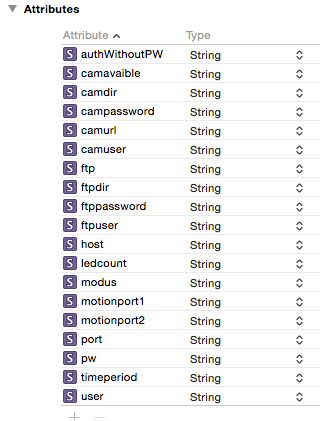
\includegraphics[width=\textwidth]{./data/entityconfig.png}
		\caption{Entität Config in CoreData}
	\end{minipage}
\end{figure}

Um einen schnellen Zugriff auf die Daten zu ermöglichen wurden Methoden zum Lesen und Schreiben implementiert. Unter anderem mit der Methode changeValueWithEntityName() kann ein Eintrag geändert werden: 
\begin{lstlisting}[caption = Implementierung CoreData-Zugriff, language=C++, frame=single, breaklines=true,columns=fullflexible, commentstyle=\color{gray}\upshape, captionpos=b, numbers = left]
func changeValueWithEntityName(entityName : String, key : String, value : AnyObject) {
    var err : NSError? = nil
    var appDel : AppDelegate = (UIApplication.sharedApplication().delegate as! AppDelegate)
    var context : NSManagedObjectContext = appDel.managedObjectContext!
    var request = NSFetchRequest(entityName: entityName)
    request.returnsObjectsAsFaults = false
    var result : Array = context.executeFetchRequest(request, error: &err)! as Array
    if (result.count == 1){
	    for res in result {
		    res.setValue(value, forKey: key)
	    }
    }
    context.save(&err)
    if (err != nil) {
	    println(err)
    }
}
\end{lstlisting}

\subsection{Konzept Synchronisation}
Beim Start der App soll die Verbindung zum Server aufgebaut werden. Hierbei sollen die Zugangsdaten überprüft werden und alle Daten synchronisiert werden (siehe Abb. \ref{fig:server-client}, folgende Seite). Das bedeutet es werden bei jeder Verbindung mit korrektem Login alle Konfigurationsdaten des Servers an den Client gesendet. Des weiteren wird der aktuelle Status der LEDs übertragen. \\
Nach dem Verbindungsaufbau ist es dem Benutzer möglich, den Modus des Systems zu verändern. Außerdem kann er alle anderen Funktionen in der App nutzen.

\begin{figure}[h]
	\begin{minipage}{\textwidth}
		\centering
		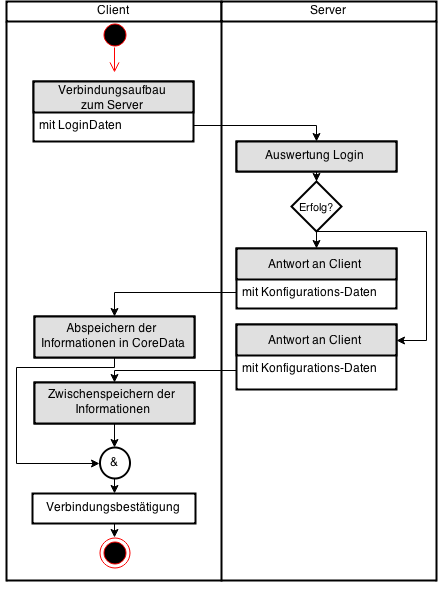
\includegraphics[width=0.6\textwidth]{./data/konzept.png}
		\caption{\label{fig:server-client}Konzept der Server-Client-Kommunikation}
	\end{minipage}
\end{figure}

\subsection{Aufbau}
\begin{wrapfigure}{r}{0.4\textwidth}
	\vspace{-20pt}
	\begin{center}
		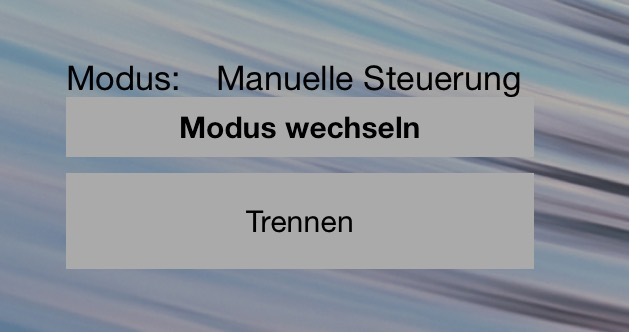
\includegraphics[width=0.35\textwidth]{./data/welcome.png}
	\end{center}
	\vspace{-20pt}
	\caption{\label{fig:welcome-image}Startseite iOS-App}
	\vspace{-10pt}
\end{wrapfigure}
In einer Standard iOS-App werden die einzelnen Seiten Klassenweise implementiert. In einem visuellen Editor können Grundelemente wie Buttons und Textfelder hinzugefügt werden. Diese werden über Outlets mit den zugehörigen Klassen verbunden und können direkt im Code angesprochen werden. 
Es wurden weitere Klassen für die Kommunikation mit der Serveranwendung und CoreData angelegt. Um zwischen den einzelnen Views zu wechseln, wird ein Menü verwendet, welches sich durch eine Wisch-\\Bewegung vom linken Rand öffnet. 

\paragraph{Startbildschirm} 
\begin{wrapfigure}{r}{0.4\textwidth}
	\vspace{-20pt}
	\begin{center}
		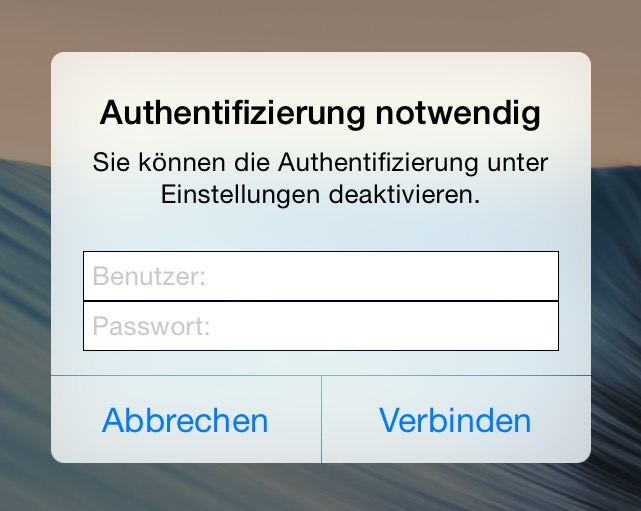
\includegraphics[width=0.35\textwidth]{./data/login.png}
	\end{center}
	\vspace{-20pt}
	\caption{\label{fig:login-image}Login iOS-App}
	\vspace{-10pt}
\end{wrapfigure}
Auf dem Startbildschirm hat der Nutzer die Möglichkeit die Verbindung zum Server herzustellen oder zu trennen (siehe Abb. \ref{fig:welcome-image}). Zusätzlich wird der aktuelle Modus des Systems angezeigt. Dieser kann auch geändert werden.\\
Wenn die App zum ersten Mal gestartet wird, ist noch keine Server-Adresse hinterlegt. Hierfür wird eine Meldung an den Benutzer ausgegeben. In diesem Fall wird statt dem aktuellen Modus der Schriftzug 'offline' gezeigt.
Der Benutzer hat die Möglichkeit die wiederholte Passwortabfrage zu deaktivieren.\\
Diese Einstellung ist in der Konfiguration zu finden.Falls dies nicht deaktiviert ist, muss bei jeder neuen Verbindung zum Server eine Eingabe der gültigen Zugangsdaten erfolgen (siehe Abb. \ref{fig:login-image}). Hierfür wird ein Login-Fenster implementiert.
\paragraph{Manuelle Steuerung} Eines der Ziele dieser Studienarbeit war die manuelle Ansteuerung der LEDs. Hierfür wurde ein View angelegt, in dem sowohl die LEDs angesteuert werden können, als auch die aktuellen Farbwerte abgerufen werden können. Über das Protokoll (siehe Kap. \ref{kapitel-protokoll}) können Farbwerte an einzelne LEDs oder auch an bestimmte Bereiche gesendet werden (siehe Abb. \ref{fig:image-colour}). Zusätzlich ist es möglich bestimmte Effekte aufzurufen\footnote{Aufgrund von mangelnder Zeit wurde nur die Ansteuerung aller LEDs implementiert. Die Effekte wurden serverseitig nur rudimentär implementiert.}. \\\\
Einzelne Farbwerte können über Farb-Buttons gesendet werden. Jedes dieser Buttons besitzt einen 'Tag', welcher den 24Bit Farbwert speichert. So wird für alle Buttons nur ein Listener benötigt. Dieser liest den Farbwert und sendet ihn, gemäß dem Protokoll, an den Server. \\
Wenn mehrere Geräte mit dem Server verbunden sind, können die Farben unabhängig voneinander gesteuert werde. Damit das jeweils andere Geräte weiß, welche Farben gerade angeschaltet sind, wurde eine Farbsynchronisation implementiert. Die Serveranwendung ruft die aktuellen Farbwerte ab und sendet sie im JSON-Format an die App. Des weiteren ist in diesem Bereich noch die Ansteuerung der Effekte möglich.\\
\begin{wrapfigure}{r}{0.4\textwidth}
	\vspace{-20pt}
	\begin{center}
		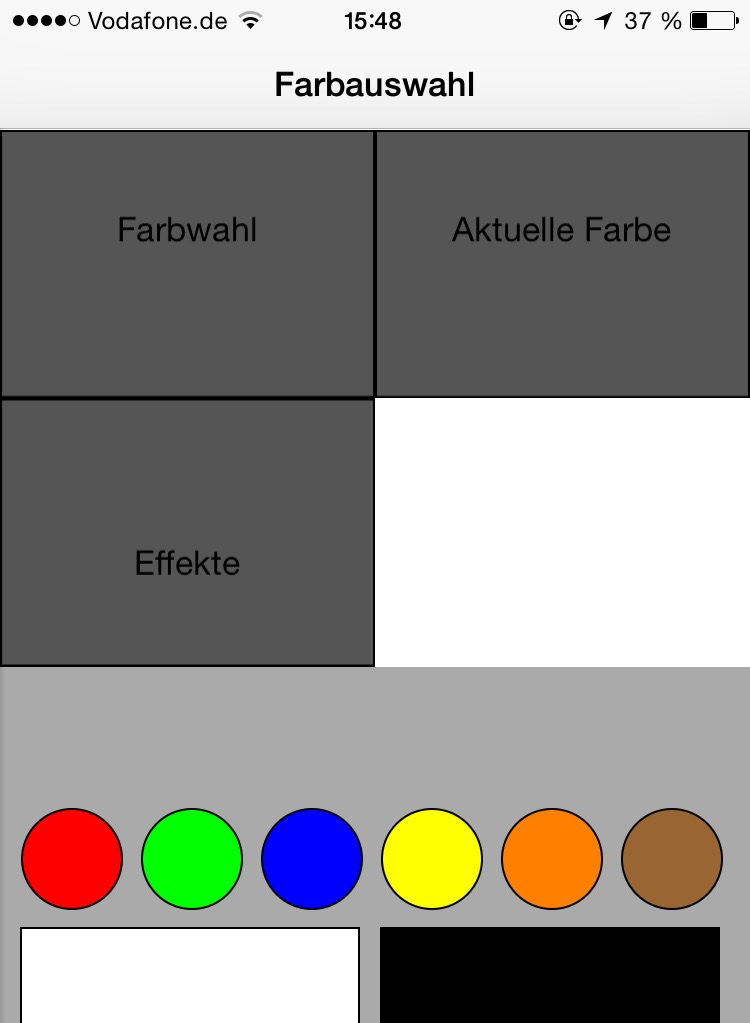
\includegraphics[width=0.35\textwidth]{./data/colour.png}
	\end{center}
	\vspace{-20pt}
	\caption{\label{fig:image-colour}Farbsteuerung iOS-App}
	\vspace{-10pt}
\end{wrapfigure}
\paragraph{Konfiguration} Während dem Betrieb der Anwendung soll kein Zugriff auf den Server notwendig sein. Die Konfiguration aller Einstellungen muss über die App möglich sein. Folgende Möglichkeiten wurden implementiert (siehe Abb. \ref{fig:image-config}): 
\begin{itemize}
	\item Grundkonfiguration: Serveradresse und Port, Anwendungbenutzer und Passwort (nicht im Bild)
	\item Hardwarekonfiguration: Änderung der Pins und Anzahl der LED
	\item Netzwerkkamera: Verfügbarkeit der Kamera und sämtliche notwendigen Einstellungen wie Adresse, Benutzer und Pfad
	\item FTP-Server: In Verknüpfung der Netzwerkkamera sind auch die FTP-Einstellungen änderbar. 
	\item Passwort: Hier wird festgelegt, ob das Passwort gespeichert wird, oder bei jeder Anmeldung neu eingegeben werden muss.
\end{itemize}
\begin{wrapfigure}{}{0.4\textwidth}
	\vspace{-100pt}
	\begin{center}
		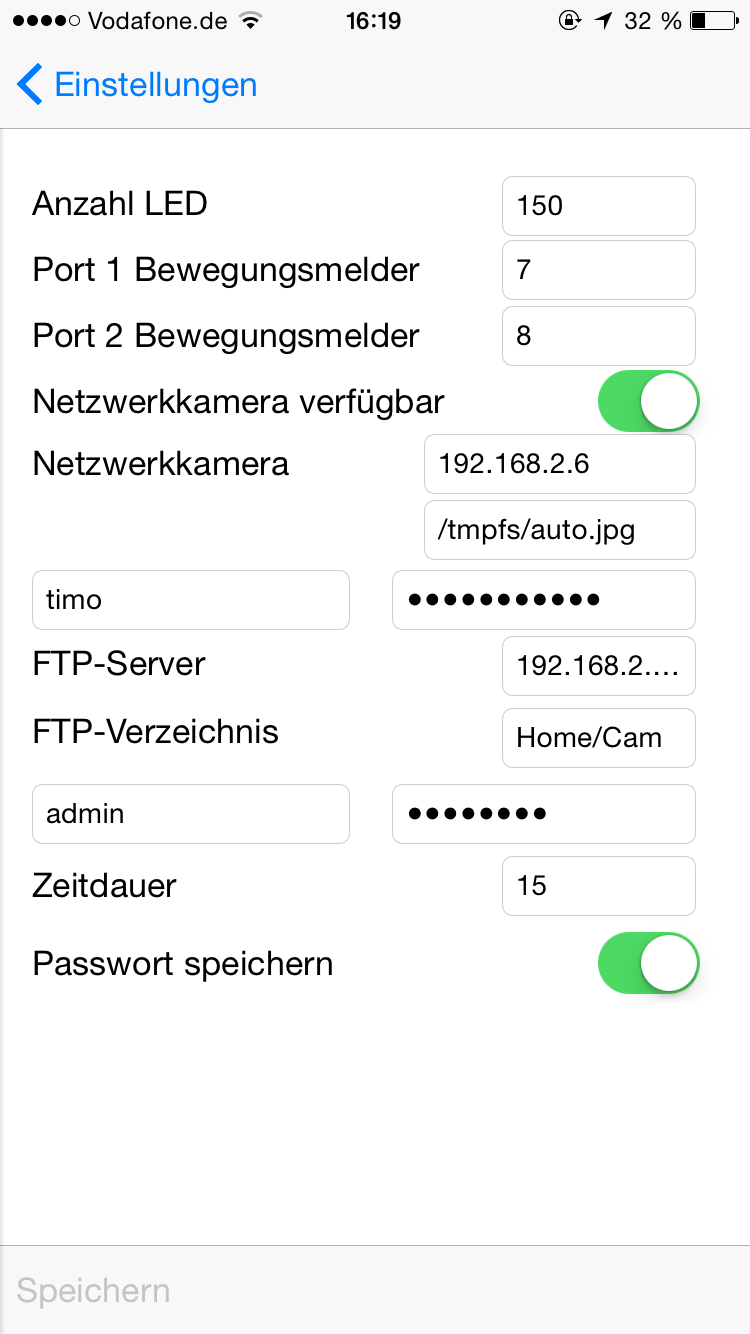
\includegraphics[width=0.35\textwidth]{./data/config.png}
	\end{center}
	\vspace{-20pt}
	\caption{\label{fig:image-config}Konfiguration in iOS-App}
	\vspace{-10pt}
\end{wrapfigure}

Die Konfiguration kann nur verändert werden, wenn eine bestätigte Verbindung zum Server besteht. Beim Öffnen der Seite wird die bestehende Konfiguration aus CoreData geladen. Beim Klick auf Speichern werden nur die veränderten Daten sowohl an den Server gesendet, als auch in der App gespeichert.\\
Wenn der Switch 'Netzwerkkamera verfügbar' deaktiviert wird, so werden alle Felder deaktiviert (ausgegraut), welche Einstellungen für die Kamera enthalten.

\clearpage
\pagebreak %Um mal wieder Ordnung in die Reihenfolge zu bringen.


\paragraph{Archiv} 
Im Archiv werden alle Bilder abgerufen, die sich auf dem FTP-Server im Verzeichnis der Anwendung befinden.
Dort werden Bilder der Netzwerkkamera gespeichert, wenn einer der Bewegungsmelder auslöst. \\
\begin{wrapfigure}{r}{0.4\textwidth}
	\vspace{-20pt}
	\begin{center}
		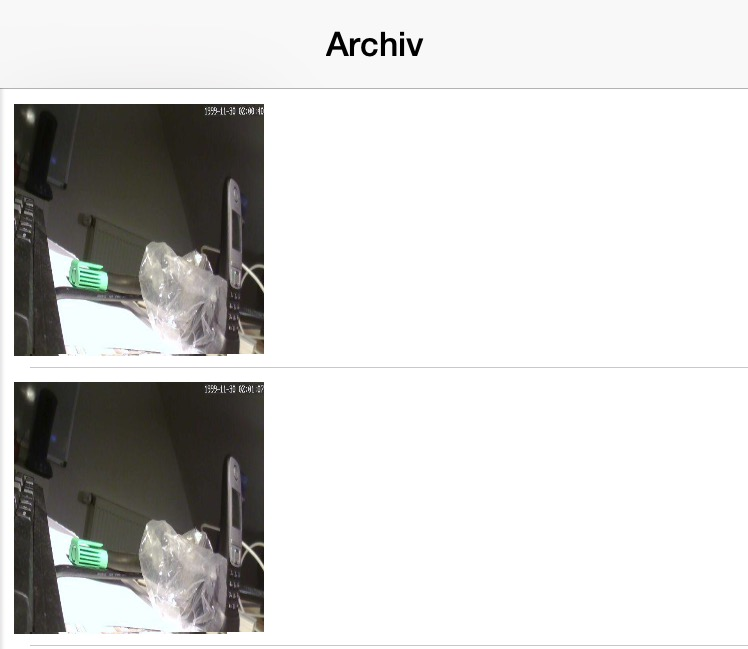
\includegraphics[width=0.35\textwidth]{./data/archiv.png}
	\end{center}
	\vspace{-20pt}
	\caption{\label{fig:image-archiv}Archiv iOS-App}
	\vspace{-10pt}
\end{wrapfigure} 

Im ersten Schritt werden die Dateinamen aus dem Verzeichnis geladen. Im zweiten Schritt werden nacheinander die Bilder geladen. Die Bilder werden in einer Tabelle angezeigt (siehe Abb. \ref{fig:image-archiv}). Damit nicht alle Bilder gleichzeitig in den View geladen werden müssen, bietet Apple das Feature 'Reusable TableView Cell'.  Dieses sorgt dafür, dass einzelne Zellen erst erstellt werden, wenn sie angezeigt werden sollen. \\
Durch einen Klick auf ein Bild kann es vergößert werden. In der vergrößerten Ansicht ist auch das Zoomen auf einzelne Bildausschnitte möglich.


\paragraph{Live} Wie sich in Kapitel \ref{subsec:kapitel-httprequest} zeigt, ist es leicht möglich über einen HTTP-Request das aktuelle Bild der Netzwerkkamera abzurufen. Mit einem Timer wird das Bild mehrfach in der Sekunde geladen, um einen näherungsweisen Live-Stream zu bieten (siehe Abb. \ref{fig:image-live}). 

\begin{wrapfigure}{r}{0.4\textwidth}
	\vspace{-20pt}
	\begin{center}
		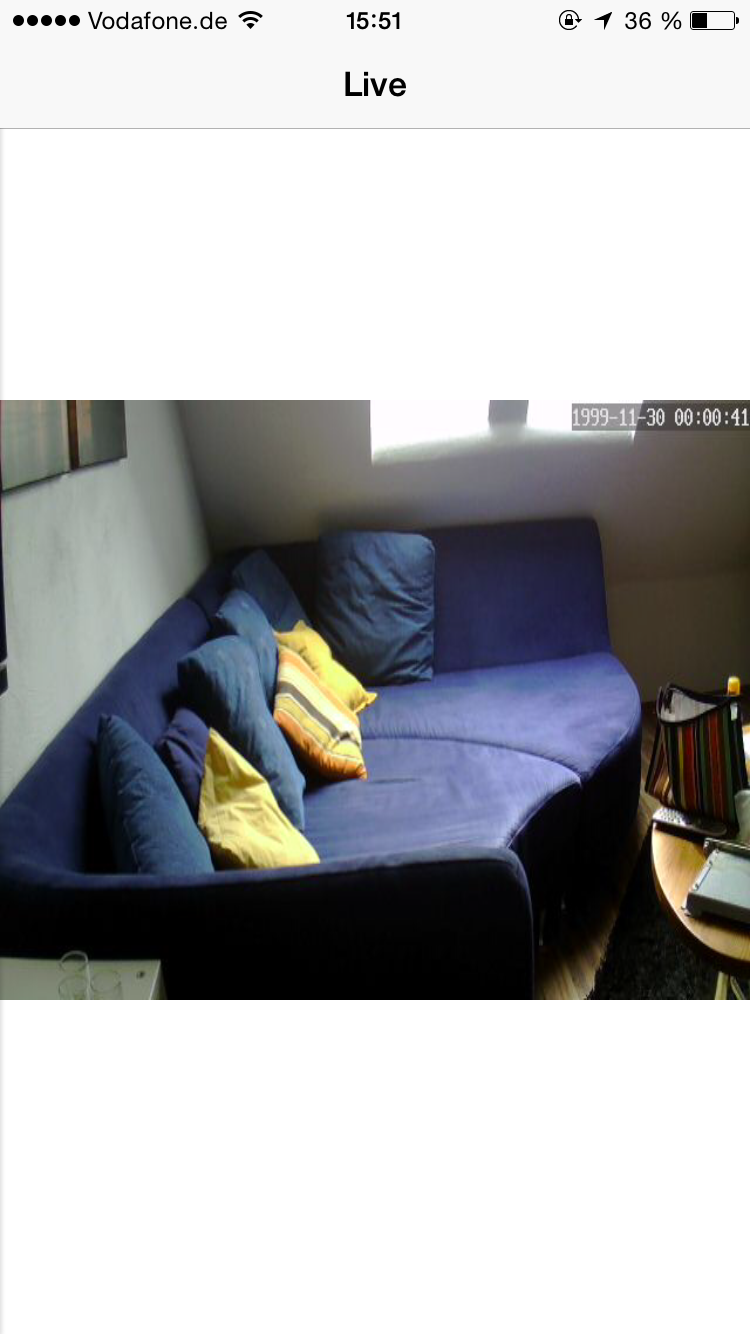
\includegraphics[width=0.35\textwidth]{./data/live.png}
	\end{center}
	\vspace{-20pt}
	\caption{\label{fig:image-live}Live-View iOS-App}
	\vspace{-10pt}
\end{wrapfigure} 




\paragraph{Framworks} Es wurden einige Frameworks eingesetzt:
\begin{itemize}
	\item \textbf{CryptoSwift}\cite{cryptoswift} Bietet viele Hashalgorithmen. \\ Autor: Marcin Krzyżanowski @krzyzanowskim
	\item \textbf{VIPhotoView}\cite{viphotoview} Notwendig für die Bildansicht im Archiv. \\ Autor: Sumi Interactive \\ Lizenz: MIT
	\item \textbf{WhiteRacoon}\cite{viphotoview} FTP-Verbindung und Management. \\ Autor: Codewise Systems \\ Lizenz: MIT
	\item \textbf{IJReachability}\cite{ijreachability} Überprüft welche Internetverbindung vorhanden ist. \\ Autor: Isuru Nanayakkara \\ Lizenz: MIT
	\item \textbf{ENSwiftSideMenu}\cite{enswiftsidemenu} Slide-Menü der Anwendung. \\ Autor: Evgeny Nazarov \\ Lizenz: MIT
\end{itemize}

